\documentclass[a4paper,12pt]{article}
\usepackage[english]{babel}
\usepackage[utf8]{inputenc}
\usepackage{t1enc}
%\usepackage[T1]{fontenc}
\usepackage{floatflt}
\usepackage{graphicx}
\usepackage{psfrag}
\usepackage{bbm}
\usepackage{amsmath}
\usepackage{amssymb}
\usepackage{slashed}
%\usepackage{showkeys}
\usepackage{hyperref}
\usepackage{ifthen}
\usepackage{subcaption}
\usepackage{epstopdf}
\usepackage{enumerate}
\usepackage{dutchcal}
\usepackage{centernot}



\hoffset=-5.0mm
\voffset=-1.9mm
%
\evensidemargin=0cm
\oddsidemargin=0cm
\topmargin=0cm%
\headheight=0cm%
\headsep=0cm%
\marginparsep=0cm%
\marginparwidth=0cm%
\textheight=24cm
\textwidth=17cm
\special{papersize=210mm,297mm}%

\def\d{\mathrm{d}}
\def\e{\mathrm{e}}
\def\imagi{\mathrm{i}}
\def\ellop{\mathop{{\sf L}}}
\def\forrasfile#1{ (see {\tt #1})}
\def\lag{{\mathcal{L}}}
\def\lap{\mathop{\Delta}}
\def\kihagy#1{}
\def\sn{\mathop{\text{sn}}}
\def\cn{\mathop{\text{cn}}}
\def\dn{\mathop{\text{dn}}}
\def\zb{\ensuremath{\bar{z}}}
\def\sign{\mathop{\text{sign}}}
\def\xii#1{\xi^{(#1)}}
\def\xij#1#2{{\xi^{(#1)}_{#2}}}
\def\op#1{{\sf #1}}
\def\tphi{\ensuremath{\tilde{\phi}}}
\def\tphi{\ensuremath{\tilde{\phi}}}
\renewcommand\Re{\mathop{\text{Re}}}
\renewcommand\Im{\mathop{\text{Im}}}
\def\Tr{\ensuremath{\mathop{\rm Tr}}}
\def\pa{\partial}


\newcommand{\doi}[1]{\href{http://dx.doi.org/#1}{DOI: #1}}%
\newcommand{\doix}[2]{\href{http://dx.doi.org/#2}{#1}}%
\newcommand{\arxiv}[2][]{%
  \ifthenelse{\equal{#1}{}}{%
    \href{http://arxiv.org/abs/#2}{\texttt{arXiv:#2}}%
  }{%
    \href{http://arxiv.org/abs/#2}{\texttt{arXiv:#2 [#1]}}%
  }%
}%


%opening
\title{Problem solutions: Statistics by R.J.~Barlow}
\author{Árpád Lukács}

\begin{document}
\maketitle

\section{Using statistics}\label{sec:UsingStatistics}

\section{Describing data}\label{sec:DescribingData}

\paragraph{2.1} The mean and the standard deviation of the data set is 19.26 and the standard deviation is 0.49.

\paragraph{2.2} With the lecturer included, the mean is 19.95 and the standard deviation is 3.44.

\paragraph{2.3} The skew in the two cases is 0.23 and 4.65, respectively.

\paragraph{2.4} The average marks in classical and quantum mechanics are 37.5 and 55.25, and the standard deviations are 25.9 and 14.2, respecitvely. The covariance matrix is
\[
 {\rm cov} =
 \begin{pmatrix}
 671.42 & 207.46\\
 207.46 & 200.69
 \end{pmatrix}
\]
and the correlation coefficient of the two variables is $\rho = 0.565$.

\paragraph{2.5} The expansion of the curtosis is
\[
 \begin{aligned}
  \gamma &= \frac{1}{\sigma^3} \overline{(x-\bar{x})^3} = \frac{1}{\sigma^3}\overline{x^3 - 3 x^2\bar{x} + 3 x\bar{x}{}^2 - \bar{x}{}^3}\\
  &= \frac{1}{\sigma^3}(\overline{x^3}-3\bar{x}\overline{x^2} + 2\bar{x}^3)\,,
 \end{aligned}
\]
where we have used the fact that the mean of a constant (such as the mean of some data) is the constant itself. The last line is eq.\ (2.14).

Similarly,
\[
 \begin{aligned}
  c &= \frac{1}{\sigma^4}\overline{(x-\bar{x})^4} - 3 = \frac{1}{\sigma^4}\overline{x^4 - 4 x^3\bar{x} + 6 x^2\bar{x}{}^2 - 4 x \bar{x}{}^3 + \bar{x}{}^4}\\
  &= \frac{1}{\sigma^4}(\overline{x^4}-4 \bar{x}\overline{x^3} + 6\overline{x^2}\bar{x}{}^2 -3\bar{x}{}^4)\,.
 \end{aligned}
\]

\paragraph{2.6} A histogram with uniform bins is
\begin{center}
 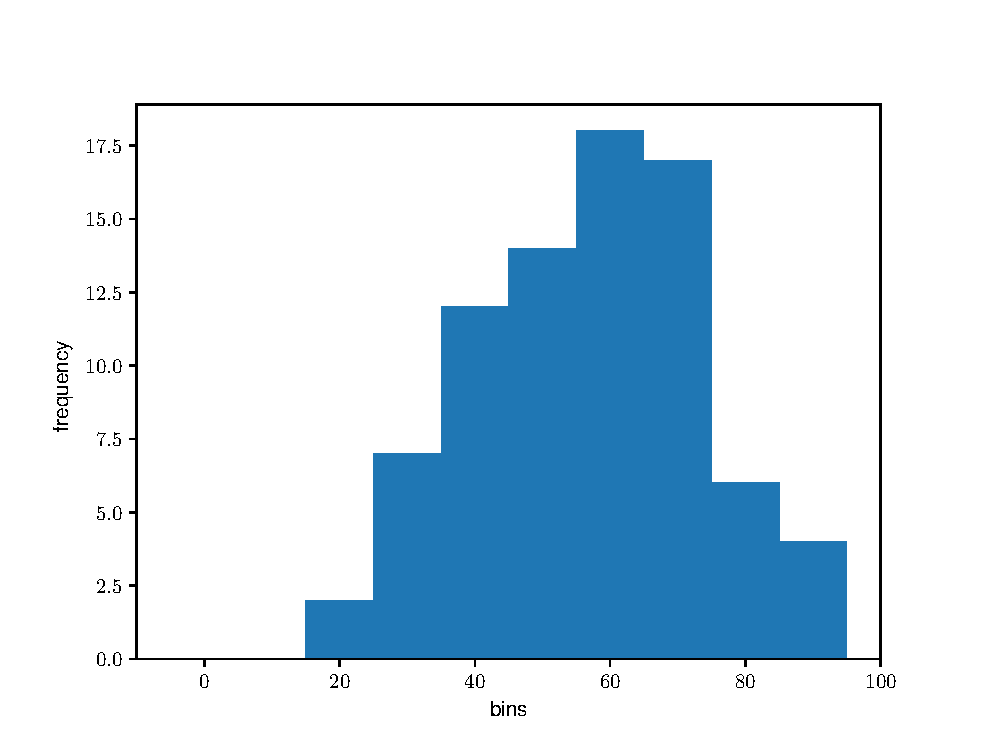
\includegraphics[scale=.5]{ca/ex2.6.eps}
\end{center}

\paragraph{2.7} The mean, median, and mode of the data in ex.\ 2.6 are 61.59, 63.5, and 79, respectively. The corresponding quantities from the histogram shown in soln.\ 2.6 are 61.75, 60-69, and 60-69.

\paragraph{2.8} The standard deviation of the data in ex.\ 2.6 is 16.67. The full width at half maximum is 40, which agrees with eq.\ (2.12), 2.25 stddev is 39.18.


\paragraph{2.9} One may form vectors of the data points of each variable, $\vec{x}_i$ containing the data points of variable $x_{(i)} - \bar{x}_{(i)}$. With this notation, the elemets of the covariance matrix are
\[
 {\rm cov}_{i,j} = \frac{1}{N}\vec{x}_i\cdot \vec{x}_j\,,
\]
and $\sigma_i^2 = \vec{x}_i \cdot \vec{x}_i / N$. According to the Cauchy-Schwarz inequality,
$|{\rm cov}_{i,j}| \le \sqrt{\sigma_i \sigma_j}$, which completes the proof, as
\[
 \rho_{i,j} = \frac{{\rm cov}_{i,j}}{\sigma_i\sigma_j}\,.
\]

\section{Theoretical distributions}\label{sec:TheoreticalDistributions}

\paragraph{3.1} Intercepting all 100 rockets has a probability of $(0.995)^{100} = 0.606$, i.e., 60.6\,\% chance. To have 50\,\% chance, we have to take the logarithm, $n \log 0.995 = \log 0.5$, yielding $n=138.2$, i.e., launching 139 rockets makes a better than even chance of hitting the target.

\paragraph{3.2} To get a better than evens chance of two rockets penetrating the defences, we have to solve
\[
 p_0 + p_1 < 1/2
\]
where $p_k = \binom{n}{k} p^k q^{n-k}$ where $p=0.005$ is the chance of hitting the target with a simple missile, and $q=1-p$, i.e.,
\[
 q^n + n q^{n-1}p < 1/2,
\]
Numerical solution yields $n>335.33$, i.e., 336 rockets have to be launched to have a better than even chance of two not being intercepted.

\paragraph{3.3} The distribution is Poisson, with an expectation value of $\lambda=15.7 \times 0.5 = 7.85$. The probability of observing less than 5 meteors is $p_0 + p_1 + \dots + p_4 = 0.1085$.

\paragraph{3.4} The Gaussian approximation to a Poission distribution with expectation value $\lambda$ is a normal distribution with expectation value and variance both $\lambda$.

Just approximating the Poisson distribution with a Gaussian, and calculating $p_0 +\dots + p_4 \approx 0.113$. Replacing the sum with the integral of the Gaussian from $-\infty$ to 4 yields 0.085 or 8.5\,\%. Table 2 can be used by realising that 4 means a deviation of $-1.37\sigma$ from the expectation value, and using the symmetry of the Gaussian.

\paragraph{3.5} The probability of still waiting after 60 cars is $(0.99)^{60} = 0.547$. As one car yields a 1\,\% chance of a lift, the expected number of drivers willing to give a lift is 0.6 per hour. The probability of no such drivers arriving in an our is, using $p_0 = \e^{-\lambda}$ (Poisson distribution) is 0.549.

\paragraph{3.6}
\begin{enumerate}[(a)]
 \item 21.87\,\%,
 \item 0.75\,\%,
 \item 13.79\,\%,
 \item 67.36\,\%,
 \item 48.35\,\%,
 \item 91.53\,\%,
 \item 0.77,
 \item 2.33.
\end{enumerate}

\paragraph{3.7} The skew of a Gaussian is
\[
 \gamma = \frac{1}{\sigma^3}\int_{-\infty}^\infty \frac{1}{\sqrt{2\pi}\sigma}(x-\mu)^3 \e^{-\frac{(x-\mu)^2}{2\sigma^2}}\d x = \frac{1}{\sqrt{2\pi}\sigma^4}\int_{-\infty}^\infty x'{}^3 \e^{-\frac{x'{}^2}{2\sigma^2}}\d x' = 0\,,
\]
as $x^3$ is odd, and the bell curve is even.

The curtosis is (after shifting the variable by $\mu$)
\[
 c = -3+\frac{1}{\sqrt{2\pi}\sigma^5}\int_{-\infty}^\infty x^4 \e^{-\frac{x^2}{2\sigma^2}}\d x=0\,,
\]
as, according to table 3.1, the integral is (using $n=2$, $a=1/2/\sigma^2$, even power), $3\sqrt{2\pi}\sigma^5$.

\section{Errors}

\paragraph{4.1} A set of 10 measurements with a resolution of 1\,mm has a resolution of $1/\sqrt{10}\,{\rm mm}\approx 0.31\,mm$, therefore, a single measurement with a resolution of 0.2\,mm is preferable.

\paragraph{4.2} The best combined measurement is weighed by the inverse squared errors, and yields
$299793105 \pm 2910\,{\rm m\,s}^{-1}$.

\paragraph{4.3} Similarly to the previous exercise, $299783690\pm 1319\,{\rm m\,s}^{-1}$.

\paragraph{4.4} The voltage is determined as $V = R \cdot I$, where $R = 1400\pm 30\,\Omega$ and $I=1120\pm 10\,{\rm mA}$, then the voltage is $V=1568\,{\rm V}$ and its error is determined by eq.\ (4.15) as $\sigma_V =V\sqrt{(\sigma_R/R)^2+(\sigma_I/I)^2} = 36\,{\rm V}$.

\paragraph{4.5} Again, using Ohm's law, and the Example on p.\ 66, $I=50\pm 1\,{\rm mA}$.

\paragraph{4.6} For $\theta=0.56\pm 0.01$, we have $\sin\theta = 0.53\pm 0.008$, $\cos\theta = 0.847\pm 0.005$, $\tan\theta = 0.63\pm 0.01$.

For $\theta=1.56\pm 0.01$ we have $\sin\theta=1\mp 10^{-4}$, $\cos\theta=0.011\pm 0.01$ and $\tan\theta=93\pm 86$. Note that in the last two cases, the errrors are so large, that the assumption of small errors breaks down, and the errors cannot be trusted, as they are calculated from a linearised assumption. Also, calculating the differences, e.g., $|\cos(\theta+\sigma_\theta) - \cos(\theta-\sigma_\theta)|$ would not make sense, as here one cannot assume that the distribution of $\cos\theta$ is still normal (the latter would work for tolerances, i.e., strict bounds for $\theta$).

\paragraph{4.7} The variance of the weighted average of eq.\ (4.6) is obtained as
\[\begin{aligned}
 \langle (\bar x - \mu)^2 \rangle &= \left\langle\left( \frac{\sum_i x_i/\sigma_i^2}{\sum_i 1/\sigma_i^2}-\mu\right)^2\right\rangle = \left\langle \left( \frac{\sum_i x_i/\sigma_i^2}{\sum_i 1/\sigma_i^2} - \frac{\sum_i \mu/\sigma_i^2}{\sum_i 1/\sigma_i^2}\right)^2\right\rangle\\
 &= \left\langle \frac{\sum_i (x_i-\mu)^2/\sigma_i^4}{(\sum_i 1/\sigma_i^2)^2} + \frac{\sum_i\sum_{j\ne i}(x_i-\mu)(x_j-\mu)/\sigma_i^2/\sigma_j^2}{(\sum_i 1/\sigma_i^2)^2}\right\rangle\\
 &= \left\langle \frac{\sum_i (x_i-\mu)^2/\sigma_i^4}{(\sum_i 1/\sigma_i^2)^2}\right\rangle = \frac{1}{\sum_i 1/\sigma_i^2}\,,
\end{aligned}\]
where we have used the fact that the $x_i$'s are uncorrelated, $\langle (x_i-\mu)(x_j-\mu)\rangle =0$ for $i\ne j$.

\paragraph{4.8} As we do not have separate error estimates for the two measurements (they come from the same source), the best is to average, yielding 406.

\paragraph{4.9} The result depends entirely on what kind of errors these are. If they are measurements based on different duration, detector efficientcy, etc., then they need to be weighted according to their number of counts (Poisson distribution), if the errors are due to errors of calibration of different detectors, according to their errors. No general answer.

\paragraph{4.10} In this case, not just the resistance is the same for the two current measurements, but the systematic error in the voltage measurements, i.e., we have $V_i = V_i' + V''$ the formar having variance $\sigma_V$, the latter having $S_V$. Then $I_i = V_i/R_i = V_i/R + V''/R$, and so the transformation matrix is
\[
 {\bf G} = \left( \frac{\partial I_i}{\partial V_j}, \frac{\partial I_i}{\partial V''}, \frac{\partial I_i}{R} \right) =
 \begin{pmatrix}
  1/R & 0   & 1/R & (V_1 + V'')/R^2 \\
  0   & 1/R & 1/R & (V_2 + V'')/R^2
 \end{pmatrix}
\]
where $(V_i + V'')/R = I_i$,
and the covariance matrix of the quantities $V_1'$, $V_2'$, $V''$, $R$ is
\[
{\bf V}_1 =
 \begin{pmatrix}
 %  V1 V2 V'' R
  \sigma_{V_1}^2 & 0 & 0 & 0 \\
  0 & \sigma_{V_2}^2 & 0 & 0 \\
  0 & 0 & S_V^2 & 0 \\
  0 & 0 & 0 & S_R^2
 \end{pmatrix}
\]
so the covariance matrix of the measurement results is
\[
 {\bf V}_2 = {\bf G} {\bf V}_1 \tilde{\bf V}_1
\]
and so %the covariance of the two measurements is
%\[
% {\rm cov}(I_1, I_2) = \frac{I_1 I_2}{R^2}S_R^2 + \frac{S_V^2}{R^2}\,,
%\]
%and
the error matrix of $I_1$, $I_2$ is
\[
 {\bf V}_2 = \frac{1}{R^2}
 \begin{pmatrix}
  \sigma_{V_1}^2 + S_V^2 - I_1^2 S_R^2 & S_V^2 + I_1 I_2 S_R^2\\
  S_V^2 + I_1 I_2 S_R^2 & \sigma_{V_2}^2 + S_V^2 - I_2^2 S_R^2
 \end{pmatrix}\,.
\]


\section{Estimation}

\paragraph{5.1} If the experiment is repeated $N$ times, then $N_S + N_F = N$, so the estimator is equivalent to $\hat\rho = N_S/N$, so the $\langle \hat\rho \rangle = \langle N_S \rangle / N = p$, so the estimator is unbiased. Also, for large $N$, the standard deviation of $N_S$ is $\sqrt{Np(1-p)}$, so that of $\hat\rho$ is $\sqrt{p(1-p)/N}\to 0$, so the estimator converges to the true value.

\paragraph{5.2} (a) The mean is 20.21. If the numbers represent measurements with a single quantity with resolution 0.8, the error on the mean is $0.8/\sqrt(7) = 0.3$.

(b) The estimate of the standard deviation assuming a known mean of 20.0 is 0.87.

(c) Estimating the standard deviation with no prior knowledge of the mean is 0.91.

(d) The error on the standard deviation estimated with no prior knowledge of the mean, using eq.\ (5.24) is 0.26. Using that to estimate the error on the mean is $0.91/\sqrt{7} = 0.34$.

\paragraph{5.3} Let us consider the average
\[
 \overline{(x-\bar{x})^3} = \overline{x^3 - 3x^2\bar{x} + 3 x\bar{x}{}^2 -\bar{x}{}^3} = \overline{x^3} - 3 \overline{x^2}\bar{x}+2\bar{x}{}^3\,.
\]
When calculating expectation values, we separate by the number of $x_i$'s that agree, e.g.,
\[
 \langle \overline{x^3}\rangle = \langle x^3 \rangle\,,
\]
and
\[
 \langle \overline{x^2}\bar{x} \rangle = \frac{1}{N^2}\left[ N\langle x^3\rangle + N(N-1) \langle x^2\rangle \langle x \rangle\right]
\]
and similarly,
\[
 \langle \bar{x}{}^3\rangle = \frac{1}{N^3}\left[ N\langle x^3\rangle + 3N(N-1)\langle x^2\rangle \langle x \rangle + N(N-1)(N-2)\langle x \rangle^3\right]\,.
\]
Putting these together yields
\[\begin{aligned}
 \langle \overline{(x-\bar{x})^3} \rangle &= \langle x^3\rangle \left[ 1 - \frac{3}{N} + \frac{2}{N^2}\right]  + \langle x^2 \rangle\langle x \rangle \left[-\frac{3(N-1)}{N} + \frac{6(N-1)}{N^2} \right] + \langle x \rangle^3 \frac{2(N-1)(N-2)}{N^2}\\
 &= \frac{(N-1)(N-2)}{N^2}\langle x^3\rangle -3\frac{(N-1)(N-2)}{N^2}\langle x^2\rangle\langle x \rangle +2\frac{(N-1)(N-2)}{N^2}\langle x \rangle^3\,.
\end{aligned}\]
Expanding the quantity to be estimated,
\[
 \langle (x-\mu)^3 \rangle = \langle x^3 \rangle -3\langle x^2 \rangle \mu + 2\mu^3\,,
\]
and noting that $\langle x \rangle = \mu$ yields the desired result that
\[
 \left\langle\frac{N}{(N-1)(N-2)}\sum_i (x_i-\bar{x})^3 \right\rangle = \frac{N^2}{(N-1)(N-2)}\langle \overline{(x-\bar{x})^3} \rangle = \langle (x-\mu)^3\rangle\,.
\]

\paragraph{5.4} We know that the expectation value is
\[
 \langle \hat V(x)\rangle = \frac{N-1}{N}(\langle x^2\rangle - \langle x \rangle^2 ) = \frac{N-1}{N}\sigma^2\,,
\]
which is calculated by expanding the bracket in $\hat V(x) = \overline{(x-\bar{x})^2}$ and separating each term into ones having $x^2$ or $x_i x_j$, $i\ne j$.

The error in the estimator is
\[
 V(\hat{V}(x)) = \langle \hat V^2 \rangle - \langle \hat V\rangle^2\,,
\]
where we assume that $N\gg 1$, and use eq.\ (5.17), to get
\[
 V(\hat V) = \frac{1}{N}\left[\langle (x-\mu)^4\rangle -\langle (x-\mu)^2\rangle^2\right]\,, 
\]
and the second one in the brackets here is $\sigma^4$, the first one, the $\sigma^4(c+3)$ according to the definition of the curtosis, eq.\ (2.15). Putting these together,
\[
 V(\hat V) = \frac{1}{N}\left[ \sigma^4(c+3) -\sigma^4\right] = \frac{\sigma^4(c+2)}{N}\,.
\]


\paragraph{5.5} Assuming that both the sine and cosine measurements have equal error $\sigma$, and are approximately of a normal distribution, the likelihood function is
\[
 L = \exp\left(\frac{-(\sin\theta-s)^2}{2\sigma^2}\right)\exp\left(-\frac{(\cos\theta-c)^2}{2\sigma^2}\right)\,,
\]
where $s$ and $c$ are the measured values of $\sin\theta$ and $\cos\theta$, respectively. The maximum likelihood condition gives
\[
 0 =\left.\frac{\partial \log L}{\partial\theta}\right|_{\theta=\hat\theta} =-\frac{(\sin\hat\theta -s)\cos\hat\theta -(\cos\hat\theta-c)\sin\hat\theta}{\sigma^2} = \frac{s\cos\hat\theta - c\sin\hat\theta}{\sigma^2}
\]
which yields
\[
 \tan\hat\theta = \frac{s}{c}\,,\quad\quad \hat\theta = \arctan\frac{s}{c}\,.
\]



\paragraph{5.6} The likelihood function is, as in the example on p.\ 82 of the book,
\[
 \log L = \sum_i \left(-\frac{t_i}{\tau}\right)-\log\tau\,,
\]
yielding the ML estimate
\[
 \hat\tau = \bar{t_i}\,.
\]
To estimate the variance, one shall calculate
\[
 V(\hat\tau) = \langle \bar t^2\rangle - \langle \bar t\rangle^2
\]
using the exponential distribution. To do this, we note that
\[
 (\bar t)^2 = \frac{1}{N^2}\left(\sum_i t_i^2 + \sum_i \sum_{j\ne i}t_i t_j\right)\,,
\]
therefore
\[
 \langle \bar{t}^2\rangle = \frac{1}{N}\langle t^2 \rangle + \frac{N-1}{N}\langle t\rangle^2
\]
yielding
\[
 V(\hat\tau) = \frac{1}{N}\left(\langle t^2\rangle + \frac{N-1}{N}\langle t\rangle^2 -\langle t \rangle^2\right) = \frac{1}{N}\frac{N-1}{N}\left( \langle t^2\rangle - \langle t\rangle^2 \right) = \frac{1}{N}\frac{N-1}{N}\tau^2\sim \frac{\tau^2}{N}\,,
\]
for $N\gg 1$.

The same result can be obtained from the MVB, the second derivative of the log likelihood function is
\[
 \frac{\d^2 \log L}{\d\tau^2} = \sum_i \left( -\frac{2 t_i}{\tau^3}\right) + \frac{1}{\tau^2}\,,
\]
the expectation value of which is $-N/\tau^2$, so for $N\to\infty$
\[
 V(\hat\tau) \sim \frac{1}{\langle -\d^2 \log L/\d\tau\rangle} = \frac{\tau^2}{N}\,.
\]

\section{Least squares}

\paragraph{6.1} The least squares fit, unsing eqs.\ (6.4, 6.5) is $v=10.1\pm 2\,{\rm mm\,s}^{-1}$. The resulting $\chi^2=3$, $\sqrt{2\chi^2}=2.46$ and the number of DoF is 6, $\sqrt{2n}=3.2$, which is OK.

\paragraph{6.2} Same fit as above, for $1/v$, yielding $v=10.1\pm 0.1 {\rm mm\,s}^{-1}$, with $\chi^2=10.6$. The $\sqrt{2\chi^2}=4.6$ and $\sqrt{2{\rm DoF}} = 3.16$.

\paragraph{6.3} In this case, $\sqrt{2/g}$ can be obtained by fitting a linear function to $t$ as a function of $x$. (a) In this case, we obtain $g \ 10.1\pm 0.09\,{\rm m\,s}^{-1}$ with a $\chi^2=23.76$, which is too large. (b) Again, fitting a linear function with non-zero intercept gives $g = 9.87 \pm 0.32\, {\rm m\, s}^{-1}$ with $\chi^2= 3.9$, which is reasonable for 3 degrees of freedom.

\paragraph{6.4} The sum of squares to be minimised is
\[
 \chi^2 = \sum_i (y_i - a x_i - b \sin x_i)^2\,,
\]
yielding the equations
\[
 \begin{aligned}
  \sum_i \left[ y_i x_i - a x_i^2 - b x_i \sin x_i\right] &= 0\,,\\
  \sum_i \left[ y_i \sin x_i - a x_i \sin x_i - b \sin^2 x_i \right] &= 0\,,
 \end{aligned}
\]
which can be written in the matrix form
\[
 \begin{pmatrix} \overline{x^2} & \overline{x\sin x} \\
  \overline{x\sin x} & \overline{\sin^2 x}
 \end{pmatrix}
 \begin{pmatrix} a \\ b \end{pmatrix}
 =
 \begin{pmatrix}
  \overline{x y} \\ \overline{y\sin x}
 \end{pmatrix}
\]
which has the solution
\[
 a = \frac{\overline{\sin^2 x}\,\overline{x y} - \overline{x\sin x}\,\overline{y\sin x}}{\overline{x^2}\,\overline{\sin^2 x} - \overline{x\sin x}^2}\,,\quad\quad
 b = \frac{\overline{x^2}\,\overline{y\sin x} - \overline{x\sin x}\,\overline{x y}}{\overline{x^2}\,\overline{\sin^2 x} - \overline{x\sin x}^2}\,.
\]
Evaluating these for the data yields $a = 1.962$ and $b = 1.036$.


\paragraph{6.5} The activity of a sample is described by
\[
 A(t) = A_0 2^{-t/\tau}\,,
\]
where $\tau$ is the half-life of the isotope. Therefore fitting a linear function $ y = m x + c$ to the logarithms of the counts,
\[
 \log c_i = \log A_0 - t_i \log 2 / \tau
\]
yields $\tau = - \log_2 / m$, and one can assume that the counts have an error of $\delta c_i = \sqrt{c_i}$, so the errors on the $\log c_i$'s are $\delta \log c_i = 1/c_i^{3/2}$, which are used as weights. This yieds $\tau = 1.034 \pm 0.007\,{\rm hours }$.



\section{Probability and confidence}

\paragraph{7.1} Make many tosses of the two coins, and register the frequencies. They converge to the expected values, the probabilities, with the deviations $\sim 1/\sqrt{N}$.

\paragraph{7.2} Apply Bayes's theorem, the following data are given, for the symptoms
\[
 \begin{aligned}
  P(\text{acute lethargy}|\text{swamp fever}) &= 1\,,\\
  P(\text{spots} | \text{swamp fever} &= 1\,,\\
  P(\text{raging thirtst}|\text{swamp fever}) &= 0.6\,,\\
  P(\text{violent sneezes}| \text{swamp fever}) &= 0.2\,,\\
 \end{aligned}
\]
for those having the illness, and
\[
 \begin{aligned}
  P(\text{acute lethargy}|\text{no swamp fever}) &= 0.1\,,\\
  P(\text{spots} | \text{no swamp fever} &= 0.03\,,\\
  P(\text{raging thirtst}|\text{no swamp fever}) &= 0.02\,,\\
  P(\text{violent sneezes}| \text{no swamp fever}) &= 0.05\,,\\
 \end{aligned}
\]
for those not having it, and the probability of having the illness is
\[
 P(\text{swamp fever}) = 10^{-4}\,.
\]
The symptoms are assumed to be independent of each other with the conditions. The aim is to calculate $P(\text{swamp fever} | \text{all symptoms})$ and $P(\text{swamp fever}| \text{all symptoms except sneezing})$. This is a case for Bayes' theorem,
\[
 P(\text{swamp fever}|\text{all symptoms}) = \frac{P(\text{all symptoms and swamp fever})}{P(\text{all symptoms})}
\]
and
\[
 P(\text{all symptoms and swamp fever}) = P(\text{all symptoms} | \text{swamp fever}) P(\text{swamp fever})
\]
and the symptoms are independent, so
\[
 \begin{aligned}
  P(\text{all symptoms}|\text{swamp fever}) &= \prod_{\text{symptoms}} P(\text{symptom}|\text{swamp fever})\,,\\
  P(\text{all symptoms}|\text{no swamp fever}) &= \prod_{\text{symptoms}} P(\text{symptom}|\text{no swamp fever})
 \end{aligned}
\]
and
\[
 \begin{aligned}
  P(\text{all symptoms}) = &P(\text{all symptoms}|\text{swamp fever}) P(\text{swamp fever})\\ &+ P(\text{all symptoms}|\text{no swamp fever}) P(\text{no swamp fever})\,.
 \end{aligned}
\]
These yield
\[
 \begin{aligned}
  P(\text{all symptoms}|\text{swamp fever}) = 0.6\times 0.2 &= 0.12\,,\\
  P(\text{all symptoms}|\text{no swamp fever}) &= 3\cdot 10^{-6}\,,\\
  P(\text{all symptoms and swamp fever}) &= 1.2\cdot 10^{-5}\,,\\
  P(\text{all symptoms}) = 1.2\cdot 10^{-5} + 2.9997\cdot 10^{-6} &= 1.5 \cdot 10^{-5}\,,
 \end{aligned}
\]
yielding
\[
 P(\text{swamp fever}|\text{all symptoms}) = 0.8\,,
\]
and similarly for all symptoms except sneezing (a.s.e.s.),
\[
 \begin{aligned}
  P(\text{a.s.e.s.}|\text{swamp fever}) = 0.6\times 0.8 &= 0.48\,,\\
  P(\text{a.s.e.s.}|\text{no swamp fever}) &= 5.7\cdot10^{-5}\,,\\
  P(\text{a.s.e.s.\ and swamp fever}) &= 4.8\cdot 10^{-5}\,,\\
  P(\text{a.s.e.s.}) &= 1.05 \cdot 10^{-4}\,,
 \end{aligned}
\]
so
\[
 P(\text{swamp fever}|\text{a.s.e.s.}) = 0.46\,.
\]


\paragraph{7.3} Performing a number of trials with $n_s$ successes and $n_f$ failures with a ratio $n_s/n_f$ is equivalent to a binomially distributed variable with ratio $r=n_s/(n_s+n_f)$. The limits on $r$ are $P_-$ and $P_+$. The ratio $n_s/n_f=r/(1+r)$, which is a monotonous function of $r$, so the limits are transformed using the same formula, into $P_-/(1-P_-)$ and $P_+/(1-P_+)$.


\paragraph{7.4} Numerically solving the equations of sec.\ 7.2.5 for a $95\,\%$ confidence level gives $P_-=0.19$ and $P_+=0.81$. Approximating the distribution with a Gaussian, that has $\mu=np=4$ and $\sigma=\sqrt{np(1-p)} = \sqrt{2}$, so the $1.64\sigma$ deviation corresponds to $1.64\sqrt{2}$, and so for the ratio, $1.64\sqrt{2}/8=0.29$, and thus the confidence interval is 0.21 to 0.79.



\paragraph{7.5} The total number of protons in the sample is $6\cdot 10^{32}$. The expected number of decays is $\log 2 / \tau$ times this number, and we wish to estimate $\tau$, the half-life. The number of decays obeys a Poisson statistic, so the confidence limits for $N_{\pm}$ can be read off from table 7.1, for a 95\,\% confidence (i.e., $P(N_- < N < N_+) = 0.9$) these are 3.29 and 13.15. The limits on the lifetime are thus come from solving $6\cdot 10^{32}\log 2/\tau_{\mp} = N_{\pm}$, yielding $\tau_{\mp} = 6\cdot 10^{32}\log 2 /N_{\pm}=3.16\cdot 10^{31}\,{\rm years}$ and $1.26\cdot 10^{32}\,{\rm years}$.

\paragraph{7.6} Both the background and the real events are Poisson-distributed, therefore, so is their sum. The measured value for the number of events here is the difference, 4 events, with the condidence interval $0.29$ to $9.15$ (subtracting the background from the limits in excercise 7.5). The resulting half-life limits are $4.10\cdot 10^{31}\,{\rm years}$ and $1.43\cdot 10^{33}\,{\rm years}$.

\paragraph{7.7} In this case, one needs to take into account that the variable is constrained. The confidence limits will be 0 and 5.15. All we know about the half-life is a lower confidence limit, $8.08\cdot 10^{31}\,,{\rm years}$.

\paragraph{7.8} We consider confidence limits. The three measurements give an average metal content of 7.5\,\%, however, the estimate for the standard deviation is 1.29\,\%. This gives an error estimate for the mean as $\sigma/\sqrt{N} = 0.65\,\%$. To evaluate significance, the $t$-value has to be obtained, $t=(\bar{x}-\mu)/(\hat{\sigma}/\sqrt(N)) = 2.94\,\%$. From table 7.2, this corresponds to a one-tailed significance level with 3 degrees of freedom between 95 and 97.5\,\%, so the result of a higher metal content is significant.


\section{Taking decisions}

\paragraph{8.1} The $\chi^2$ obtained using eq.\ (8.6) from the data in the table in sec.\ 3.3.1 is 0.71. The degrees of freedom is 4, i.e., the fit is extremely good, $\chi^2 \ll {\rm DoF}$.

\paragraph{8.2} $\chi^2$ is 3313 with the data point 1 for 9 events, and 3.24 with that left out (replaced by 0 events). The number of degrees of freedom is 9 and 8, respectively(10 points, 1 parameter, $\lambda$, and in the second case, one outlier removed). For the expectation value of the Poisson distribution we get 0.777 and 0.774.

\paragraph{8.3} In these cases,
\begin{enumerate}[(a)]
 \item At the 10\,\% significance level, the efficiency of 90\,\% is accepted. At any smaller significance, it would be rejected.
 
 \item In this case, the probability of 3 failures out of 3 is 0.001, so at any significance larger than this, the hypothesis is rejected.
  
 \item Of 10 tries, there is a 7\,\% probability of 3 or more failures. At a 10\,\% significance, the advertised efficiency is rejected. At any significance $\le$ 7\,\% it is accepted.
 
 \item We reject the efficiency. At least 30 errors has a probability of $2\cdot10^{-8}$.
\end{enumerate}
For choosing $N$, it is necessary to decide with what precision we want to detect an efficiency below 90\,\%. For $N$ large, for the failures, we may approximate the binomial distribution with a normal with expectation value $\mu = Nq$ and standard deviation $\sigma = \sqrt{Npq}$, where $q=1-p$, and $p$ is the efficiency. For a given $p$, a number of failures larger than $\mu + 1.64 \sigma$ has $< 10\,\%$ probability. E.g., we can distinguish a detector with efficiency $p$ from a 90\,\% efficient one if $\mu + 1.64 \sigma > 0.1 N$. This can be used to choose $N$.

\paragraph{8.4} The average temperature is $10.12 \pm 0.06$ (not given in the book whether C or K). Assuming it is constant yields $\chi^2 = 14.9$, which corresponds to a probability sligthly above 10\,\% for DoF 9, in table 8.1, so the hypothesis is rejected at 10\,\% significance. Assuming the true value is 10.1 yields $\chi^2 = 15$, which is accepted (now DoF is 10).

\paragraph{8.5} The fit receives 25 input data points, the Gaussian has 3, and the flat background 1 parameters, so the DoF is 21.

\paragraph{8.6} The variance is usually estimated as
\[
 \hat V = \frac{1}{N}\sum_k (x_k - \bar{x})^2\,,
\]
when the binning is done, $x_k$ is replaced by the value at the center of the bin, $x_j$, where $j=j(k)$ is the bin to which it belongs, and
\[
 (x_k - \bar{x})^2 = (x_j + \xi_k - \bar{x})^2 = (x_k-\bar{x})^2 + 2 \xi_k (x_k-\bar{x}) + \xi_k^2\,,
\]
the first term yields the binned approximation in the book. If one assumes that the points are uniformly distributed within the bin, the second one averages out to zero, and the third one to $\int_{x_j-w/2}^{x_j+w/2}\xi_k^2 P(x)\d x / \int_{x_j-w/2}^{x_j+w/2}P(x)\d x \approx w^2/12$.


\section{Ranking methods}


\paragraph{9.1} The total number of pairs $xy$ where $x$ is from sample $X$ and $y$ from $Y$ is $N_x N_y$. In each case (if there are no ties), either $x$ is after $y$ contributing to $U_x$ or the $y$ before $x$, contributing to $U_y$. This proves eq.\ (9.1).

If the two samples are ranked together, the ranke of a given element (say, $x$) is the number of $x$'s and the number of $y$'s before it. The latter ones are those that do not each contribute one to $R_x$, while the former not. The total contribution of the $x$'s to $R_x$ is $N_x(N_x-1)/2$, so $R_x - N_x(N_x-1)/2$ is the sum of all $y$'s before $x$'s, of all $N_x N_y$ comparisons these are the ones not contributing to $U_x$, yielding
\[
 U_x = N_x N_y - (R_x - N_x(N_x-1)/2)\,,
\]
proving eq.\ (9.2).


\paragraph{9.2} (a) In the run test, we find that the letter sequence is b b b a a b a b a b b b a a a a a, the number of runs is 8. The expected number is 9.47, with a variance of 3.96, the deviation is 0.74 standard deviation, corresponding to a probability of 54.05\,\%. The two samples agree. (b) The resulting total numbers of preceded elements from the other samples are $U_a = 17$, $U_b = 55$, for $U_a$ the expectation is 36, with a variance of 102, so the deviation is 1.88 standard deviations, corresponding to a 93.99\,\% probability, rejected at the 10\,\% confidence.

\paragraph{9.3} (a) In this case the sequence for the run test is a a a a a b b b b b b b b b b a a a a a with 3 runs. The expected number of runs is  11, with a variance of 4.74, the deviation is 3.68 standard deviations, so the hypothesis of coming from the same distribution is rejected. (b) In the Mann-Whitney test $U_a=50$, $U_b=50$, and the expectation is 50 with a cariance of 166.7, so the Mann-Whitney test accepts the samples.

Note that sample ``a'' tends to avoid the true value of 1000. Maybe the seller sold the best ones separately.

\paragraph{9.4} Pearson's correlation coefficient is 0.712, Spearman's is 0.782, and the $T$ value in Wilcox\-on's matched pairs signed rank test is 36 with an $N$ of 14. Not significant at any level in table 9.1.

The interpretation might be that the political opinion of husband and wife is correlated, both if the numerical scale is taken seriously (Pearson) and if only the ranking (Spearman). Wicoxon's test refutes the hypothesis that the two distributions are the same, i.e., opinion of husband and wife are correlated but not the same. 


\section*{Notes}
\paragraph{p.\ 23} The book says that ``expectation values \dots do not multiply \dots unless [the two random variables] are independent''. This is imprecise. The expectation values multiply if the two variables are independent, but the variables may well be dependent (i.e., their probability distribution function $P(f=a, g=b) \ne P(f=a) P(g=b)$), just uncorrelated (which is a word for the expectation values to multiply). There are many examples, e.g., let $x$ be an integer random variable with any distribution such that $P(x=n) = P(x=-n) = p_n$, and $f=x$ and $g=|x|$. These are clearly not independent,
\[
 P(f=k, g=\ell) = \left\{
 \begin{aligned}
  &P(f=k) = p_k\,,\text{\ if } \ell=|k| \\
  &0\,,\hspace{5.8em}\text{\ otherwise}
 \end{aligned}
 \right.
\]
still,
\[
 \langle f\cdot g\rangle = \sum_{n} n |n| p_n = \sum_{n>0} n^2 p_n + \sum_{n<0} n|n| p_n = \sum_{n>0} (n^2 + (-n)|-n|) p_n = 0\,,
\]
and $\langle f\rangle = 0$, $\langle g \rangle =\sum_{n>0}2n p_n > \sum_{n>0} p_n = 1/2$, and $\langle f \rangle \langle g \rangle = 0$.
\emph{Independence is a stronger property of two random variables than uncorrelatedness.}


\paragraph{p.\ 80} In eq.\ (5.25b), in stead of $1/(N-1)$, Bessel's correction should be a factor of $N/(N-1)$ and the replacement $\sigma_i \to s_i$ w.r.t.\ (5.25a).


\end{document}

